\section{Reiezione di Banda o Notch}
La struttura del filtro notch, riportata in Fig. \ref{fig:circuito}, attenua l'ampiezza di segnale solo per una determinata frequenza, detta anche in questo caso di risonanza ($\nu_0=\frac{1}{2 \pi \sqrt{LC}}$), alla quale la serie di capacità e induttanza avrà impedenza complessiva nulla. Considerando come valori di $R$, $L$ e $C$ le stesse del circuito passa banda, riportiamo le leggi teoriche calcolate:\\

\noindent
\begin{minipage}{.5\linewidth}
\begin{equation}
\frac{|V_{out}|}{|V_{in}|}=\sqrt{\frac{\left(C L \omega ^2-1\right)^2}{C \omega ^2 \left(L \left(C L \omega ^2-2\right)+C R^2\right)+1}}
\label{notchGain}
\end{equation}
\end{minipage}%
\begin{minipage}{.5\linewidth}
\begin{equation}
\phi=arctan\left[\frac{C R \omega}{C L \omega ^2-1}\right]
\label{notchPhi}
\end{equation}
\end{minipage}
\break

Come osserviamo dal diagramma di Bode (Fig. \ref{fig:notch}), per questo circuito la legge teorica non è compatibile per alte frequenze in nessuno dei due grafici. I dati sembrano infatti seguire una legge ben diversa da quella stimata. Inizialmente abbiamo pertanto risolto analiticamente il circuito considerando anche la resistenza parassita interna all'induttanza, come nel caso del filtro passa banda. La legge ricavata ha ridotto la discrepanza tra previsione teorica e dati sperimentali solo per le frequenze vicine a $\nu_0$, ma non ad alte frequenze.

Le formule ricavate sono le seguenti:\\

\noindent
\begin{minipage}{.5\linewidth}
{\small
\begin{equation}
\frac{|V_{out}|}{|V_{in}|}=\sqrt{\frac{C \omega ^2 \left(L \left(C L \omega ^2-2\right)+C R_L^2\right)+1}{C R_L^2 \left(L \left(C L R_L^2-2\right)+C (R+R_L)^2\right)+1}}
\label{eq:notchGain_corr}
\end{equation}
}
\end{minipage}%
\begin{minipage}{.5\linewidth}
{\small
\begin{equation}
\phi=arctan\left[\frac{C R \omega \left(C L \omega ^2-1\right)}{C \omega ^2 \left(L \left(C L \omega ^2-2\right)+C R_L (R+R_L)\right)+1}\right]
\label{eq:notchPhi_corr}
\end{equation}
}
\end{minipage}\\

Abbiamo dunque cercato un motivo di tale incompatibilità. Dai dati sembra che per alte frequenze ci sia qualcosa che smorza l'intensità del segnale e ne cambia la fase. Abbiamo dunque avanzato varie ipotesi.

\begin{wrapfigure}[32]{r}[0pt]{115mm}
%	\centering
    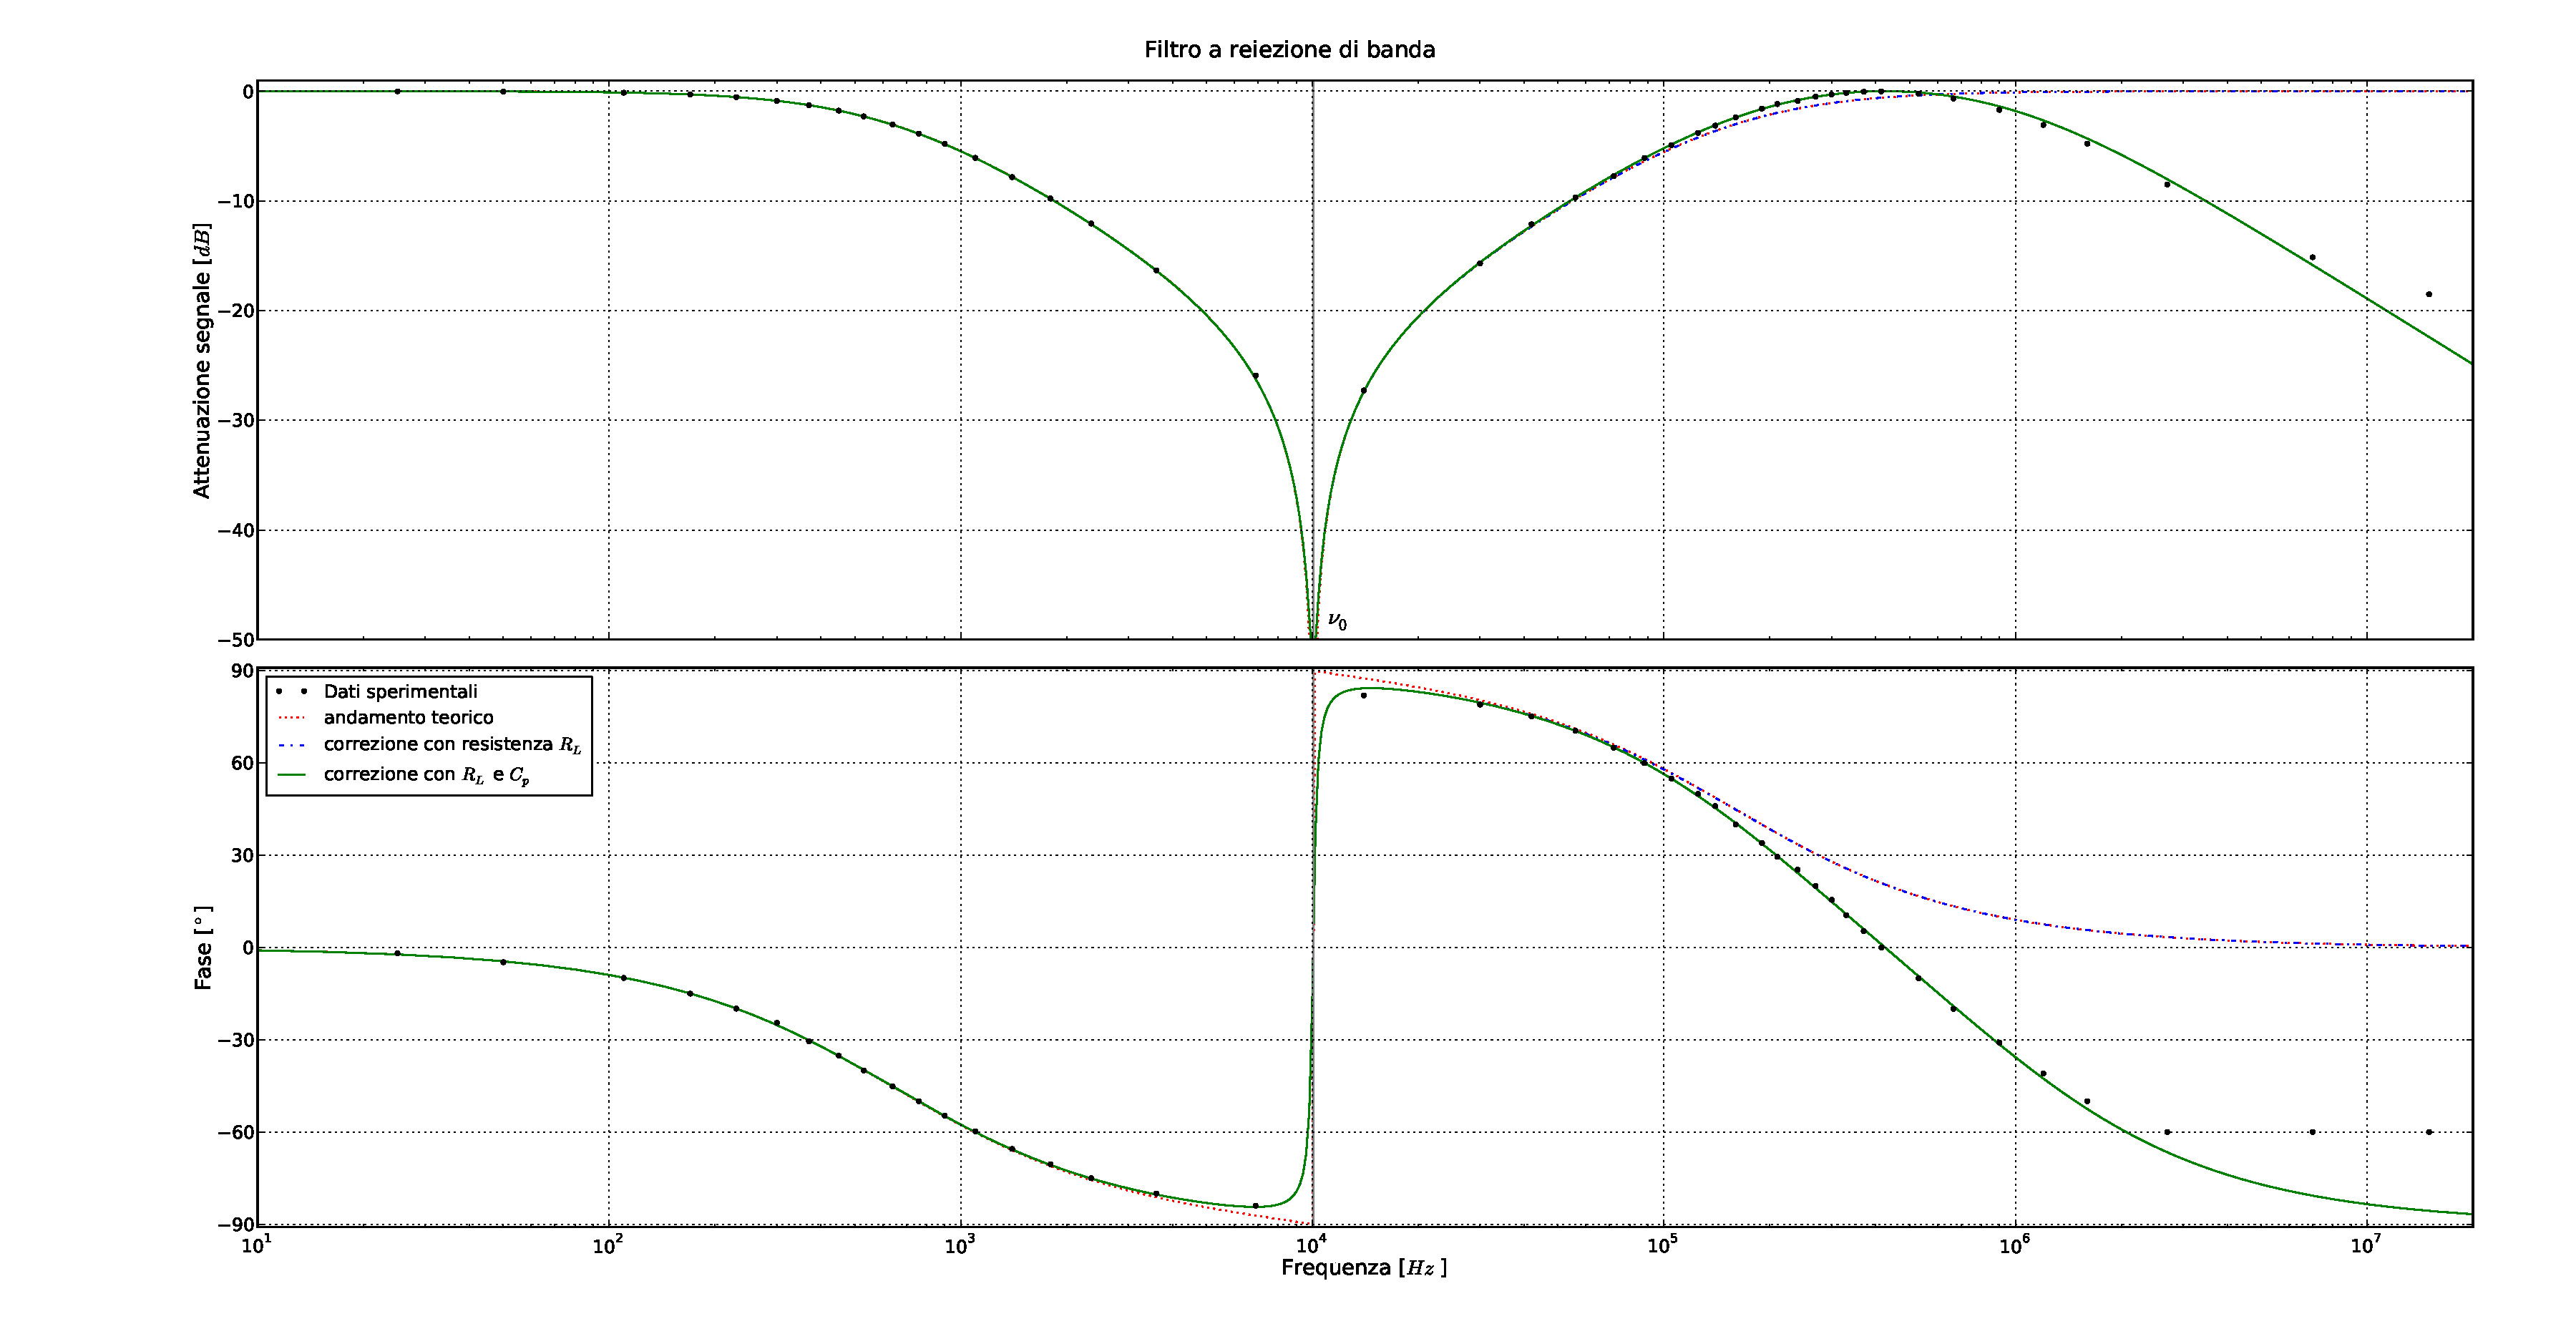
\includegraphics[width=120mm]{notch.pdf}
    \caption{Diagrammi di Bode per il filtro a reiezione di banda.}
    \label{fig:notch}
\end{wrapfigure}


Come si vede graficamente, considerare la sola esistenza della resistenza relativa all'induttanza non è sufficiente per correggere il modello teorico da noi adottato.
Poiché il comportamento ad alte frequenze è simile a quello del filtro passa basso, la prima idea che ci è venuta è stata quella di provare ad aggiungere in parallelo all'induttanza un condensatore. Così facendo, infatti, ci si trova in una configurazione tale per cui il segnale per alte frequenze subisce uno smorzamento. Sono state dunque calcolate le leggi teoriche per il circuito mostrato in Fig. (??), eseguendo poi un fit numerico per trovare dei valori di una possibile capacità parassita $C_p$ che rendesse compatibile la legge ipotizzata. Ricordiamo che tale scelta è del tutto arbitraria e sarà discussa nelle conclusioni. Il valore stimato della capacità parassita risulta essere $C_p \approx 140 \si{\pico\farad}$. Abbiamo notato che variando il valore di $C_p$ di $10 \si{\pico\farad}$ la legge teorica non era compatibile per eccesso o per difetto rispetto ai dati sperimentali nella fascia di frequenze più alte. Non possiamo dunque stimare l'incertezza su $C_p$ partendo dai dati da noi rilevati. Le equazioni da noi trovate sono:

 
\noindent
%\begin{minipage}{.5\linewidth}
{\tiny
\begin{equation*}
\frac{|V_{out}|}{|V_{in}|}=\sqrt{\frac{\omega ^2 (C+C_p) \left(L \left(L \omega ^2 (C+C_p)-2\right)+R_L^2 (C+C_p)\right)+1}{\omega ^2 \left(C^2 \left(R^2 \left(C_p \omega ^2 \left(L \left(C_p L \omega ^2-2\right)+C_p R_L^2\right)+1\right)+L^2 \omega ^2+2 R R_L+R_L^2\right)+2 C \left(L \left(C_p L \omega ^2-1\right)+C_p R_L^2\right)+C_p \left(L \left(C_p L \omega^2-2\right)+C_p R_L^2\right)\right)+1}}
\label{eq:notchGain_corr2}
\end{equation*}
}
%\end{minipage}%
%\begin{minipage}{.5\linewidth}
{\tiny
\begin{equation*}
\phi=arctan\left[\frac{C R \omega \left(-C_p L^2 \omega ^4 (C+C_p)+\omega ^2 \left(L (C+2 C_p)-C_p R_L^2 (C+C_p)\right)-1\right)}{\omega ^2 \left(C^2 R R_L-2 L (C+C_p)+R_L^2 (C+C_p)^2\right)+L^2 \omega ^4 (C+C_p)^2+1}\right]
\label{eq:notchPhi_corr2}
\end{equation*}
}
%\end{minipage}
\break





